\subsection{Convex Hull Trick}

Convex Hull Trick is an algorithm to find $\min_{j < i}(f_j(x))$ or $\max_{j < i}(f_j(x))$ efficiently.

First, we convert the function $f(x)$ to $mx+c$, which $x$ depends only on $i$, $m$ and $c$ depends only on $j$. For example

\begin{lstlisting}
dp[i] = max(dp[j] + x[i]*y[i] - x[j]*y[i] - a[i])
      = max((-x[j])*y[i] + dp[j]) + x[i]*y[i] - a[i]
\end{lstlisting}

As we can see, m = -x[j], x = y[i], c = dp[j]. Note that if we want to do CHT, the slope \textbf{must} be monotonic. Otherwise, we have to use Li-Chao Tree.

Now, how do we compute the maximum or minimum? We know that the recurrence is a line with monotonic slope.

\subsubsection{Inserting}

We will use \texttt{deque <int>} to store the lines indices.

For computing maximum, we want to maintain the lines as lower hull shaped. For minimum, we want the lines as upper hull shaped.

Before inserting, we have to check whether the old line is useless or not. We can do that by checking the intersection point between the [new line, top] and [top, top-1]. (You should try drawing on paper by yourself.)

\begin{figure}[h]
    \centering
    \begin{minipage}{0.4\textwidth}
        \centering
        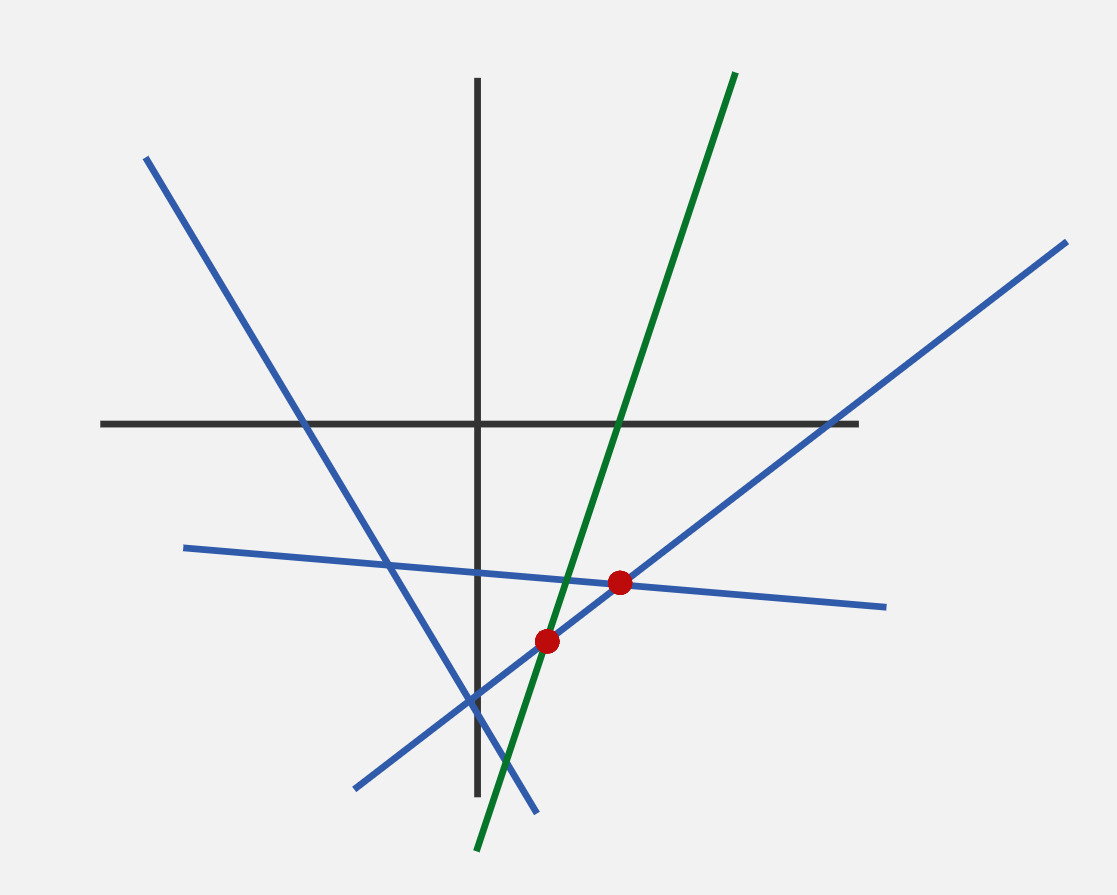
\includegraphics[width=\textwidth]{assets/cht_max.jpg}
        \caption*{Lower Hull (Maximum)}
    \end{minipage}
    \hfill
    \begin{minipage}{0.4\textwidth}
        \centering
        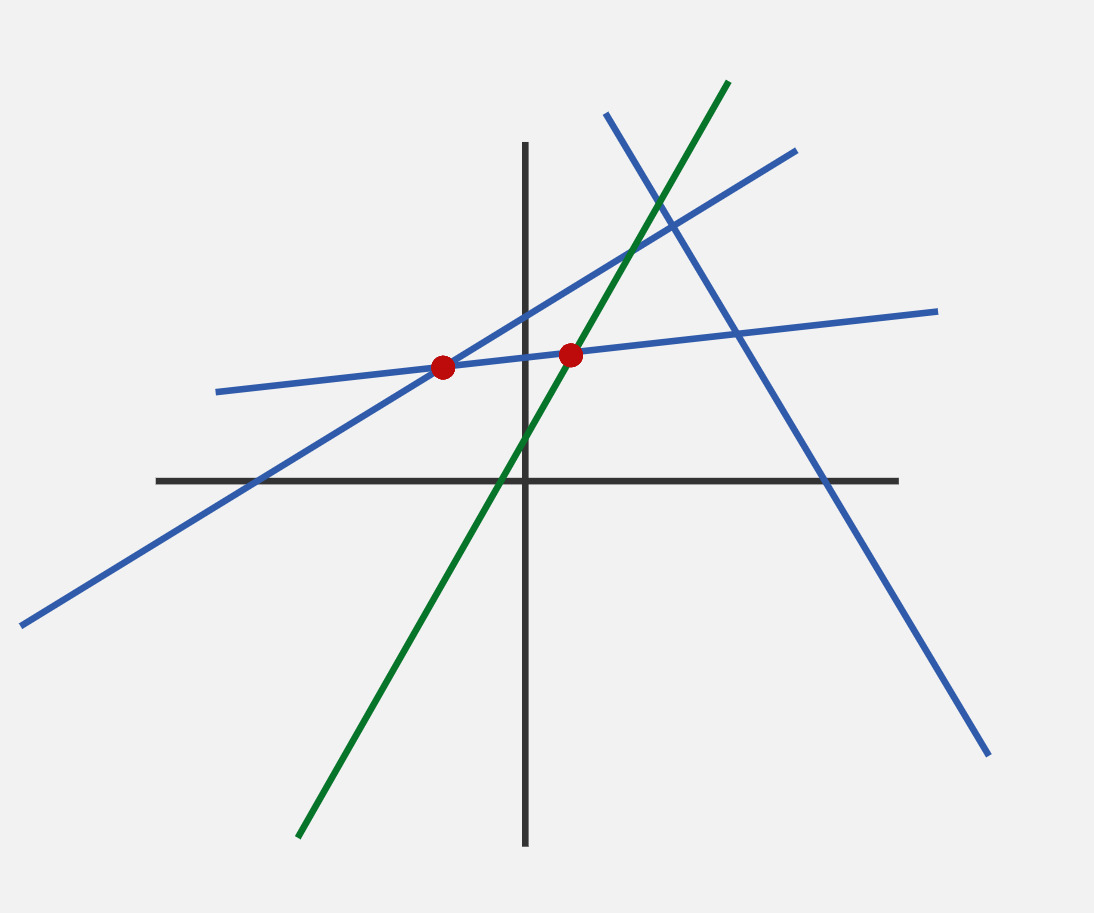
\includegraphics[width=\textwidth]{assets/cht_min.jpg}
        \caption*{Upper Hull (Minimum)}
    \end{minipage}
\end{figure}

For finding the intersection point we can do

\begin{lstlisting}
double m(int x, int y) {
    return (double) (c[x] - c[y]) / (m[y] - m[x]);
}
\end{lstlisting}

\subsubsection{Querying}

\textbf{Monotone Query}

If the hull is maintained correctly for each type of query, we will always query from front for non-decreasing queries, and always from back for non-increasing queries.

We will check the top and top-1. For maximum, if $f_\text{top}(x) \le f_\text{top-1}(x)$, we pop the top. For minimum, if $f_\text{top}(x) \ge f_{\text{top-1}}(x)$, we pop the top. For example

\begin{lstlisting}
while (sz > 1 && calc(cht[0], p[i]) <= calc(cht[1], p[i])) {
    cht.pop_front(), sz--;
}
\end{lstlisting}

Then the answer will be $f_\text{top}(x) + c$ where $c$ is a constant that depends only on $x$.

\noindent\textbf{Arbitrary Query}

We perform a binary search for the line that contain $x$.

\begin{figure}[h]
    \centering
    \centering
    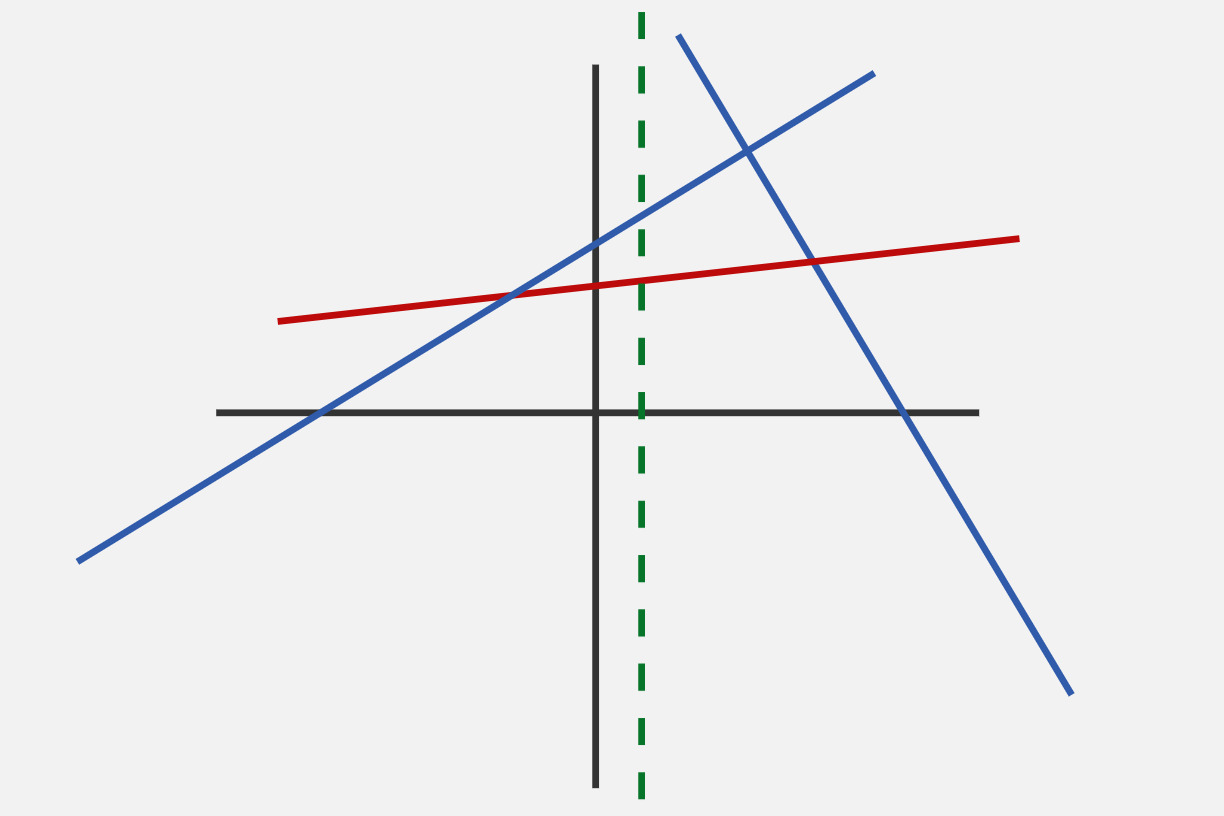
\includegraphics[width=0.6\textwidth]{assets/cht_qry.jpg}
\end{figure}

\begin{lstlisting}
int l = 0, r = sz-2, idx = sz-1;
while (l <= r) {
    int mid = l + (r-l)/2;
    if (m(cht[mid], cht[mid+1]) <= x) l = mid+1;
    else r = mid-1, idx = mid;
}
\end{lstlisting}

\break